\subsection{A whole-beam clearance certificate for the same magnetic model}
\label{sec:unifiedsafety}
The conservative normal form and the safety calculation use the same
clamped-free beam, static field, magnetic dipole, and energy.  Safety is a
statement about the driven physical equations, with their nonnegative drag;
it does not require a driven trajectory to lie on a conservative KAM torus.
For the planar, small-slope model, write $w(s,t)$ for transverse
displacement, $m=\rho A$ for line density, $c_d\geq0$ for distributed viscous
drag, and $\vartheta=w_s(L,t)$ for the tip slope used in the dipole potential.
The equations and natural end conditions are
\begin{align}
 m w_{tt}+c_d w_t+EIw_{ssss}&=0,\qquad 0<s<L,\\
 w(0,t)=w_s(0,t)&=0,\qquad w_{sss}(L,t)=0,\\
 EI w_{ss}(L,t)&=\mu\{B_y(t)\cos\vartheta-B_0\sin\vartheta\}.
 \label{eq:unifiedbeamportBC}
\end{align}
The end moment is the derivative of the same cosine potential used to
generate the training trajectories.  In particular, the varying transverse
field is an input port, not an additional autonomous Hamiltonian perturbation.
For a sufficiently regular solution satisfying the mechanical power identity,
the stored energy relative to the aligned static-field equilibrium is
\begin{align}
 E(t)&=\frac12\int_0^L\{m w_t^2+EIw_{ss}^2\}\dd s
        +\mu B_0(1-\cos\vartheta),\\
 \dot E&=-c_d\int_0^L w_t^2\dd s
             +\mu B_y\cos\vartheta\,\dot\vartheta.
 \label{eq:unifiedSIpower}
\end{align}
All inequalities below also hold for the conforming cubic-Hermite finite
element (FE) system and any of its Galerkin subspaces, because their energies
are the restrictions of this expression and retain the same input power.
In the balanced coordinates of the learning experiment, $E=\mu B_0 h_*$
for the physical target energy,
$\vartheta=d^{\mathsf T}X$, and the port force in the $Y$ equation is
$d(B_y/B_0)\cos(d^{\mathsf T}X)$.

\begin{proposition}[Clearance and field-variation budget]
\label{prop:unifiedvariation}
Assume $B_0>0$, $c_d\geq0$, and an absolutely continuous applied field
$B_y$ on $[0,T]$.  Define
\begin{align}
 S_T&=\sup_{0\leq t\leq T}|B_y(t)|+|B_y(0)|\notag\\
    &\quad+\int_0^T|\dot B_y(t)|\dd t,\\
 C_T&=\mu\sqrt{\frac{2L}{EI}}S_T,
 \\
 R_T&=\frac{C_T+\sqrt{C_T^2+4E(0)}}{2}.
 \label{eq:unifiedvariationbudget}
\end{align}
Then, throughout $[0,T]$,
\begin{equation}
 \begin{aligned}
 E(t)&\leq R_T^2,\\
 |w(s,t)|&\leq\sqrt{\frac{2s^3}{3EI}}R_T,\\
 |w_s(s,t)|&\leq\sqrt{\frac{2s}{EI}}R_T.
 \end{aligned}
 \label{eq:unifiedcontinuumshape}
\end{equation}
For a straight corridor with wall half-width $a$ and rod radius $r$, let
$c=a-r>0$.  A sufficient condition for positive clearance of the whole
rod is $R_T<\sqrt{E_c}$, where
\begin{equation}
 E_c=\frac{3EIc^2}{2L^3}.
 \label{eq:unifiedclearanceenergy}
\end{equation}
For $E(0)<E_c$, the following directly checkable operating condition is
equivalent to this sufficient energy condition:
\begin{equation}
 S_T<\frac{E_c-E(0)}{\mu\sqrt{2LE_c/EI}}.
 \label{eq:unifiedoperationbudget}
\end{equation}
These conclusions hold for every nonnegative drag coefficient, including zero.
\end{proposition}

\begin{proof}
Since $B_0>0$, the static magnetic energy is nonnegative and
$\|w_{ss}\|_{L^2}^2\leq2E/EI$.
The clamped conditions imply
$w(s)=\int_0^s(s-\xi)w_{ss}(\xi)\dd\xi$ and
$w_s(s)=\int_0^s w_{ss}(\xi)\dd\xi$.
Cauchy--Schwarz gives the two spatial inequalities in
\eqref{eq:unifiedcontinuumshape} with $\sqrt E$ in place of $R_T$.
Write $D_c(t)=\int_0^t c_d\|w_t\|_{L^2}^2\dd\tau$.
Integrating \eqref{eq:unifiedSIpower} by parts in the input term gives
\begin{align*}
 &E(t)+D_c(t)-E(0)\\
 &\quad=\mu B_y(t)\sin\vartheta(t)\\
 &\qquad-\mu B_y(0)\sin\vartheta(0)\\
 &\qquad-\mu\int_0^t\dot B_y(\tau)\sin\vartheta(\tau)\dd\tau.
\end{align*}
Set $M_T=\sup_{[0,T]}\sqrt{E(t)}$.
Using $|\sin\vartheta|\leq|\vartheta|
\leq\sqrt{2L/EI}\,M_T$ and discarding the nonnegative dissipation yields
$M_T^2\leq E(0)+C_TM_T$.
The positive root is $R_T$.
The entire radius-$r$ tube about the centerline remains between the walls
when $\sup_s|w(s,t)|<a-r$.
Solving $R_T<\sqrt{E_c}$ gives
\eqref{eq:unifiedoperationbudget}.
\end{proof}

For a nonuniform planar corridor, let $c(s)>0$ be the Euclidean distance
from the undeformed point $(s,0)$ to the wall, less the rod radius.
The distance-to-wall function is one-Lipschitz, so $|w(s)|<c(s)$
keeps the radius-$r$ tube clear. The same argument replaces $E_c$ by
$\inf_{0<s\leq L}3EIc(s)^2/(2s^3)$.
For an inclined or curved wall, a local vertical half-width is not
a substitute for this Euclidean clearance.
This sufficient condition applies to the specified corridor geometry;
vessel-specific use requires its own wall data. The continuum inequality
applies directly to solutions with the stated initial-energy and
applied-field bounds, and holds separately for conforming FE solutions.
It therefore requires neither a two-mode reconstruction error estimate
nor an identification of an FE trajectory with a continuum solution.

For the shared SI parameters, choose $a=4.6$ mm and $r=0.6$ mm, so that
$c=4$ mm.  The resulting $E_c$ is $23.8565$ nJ.
For a monotone field ramp from zero to $A$ followed by a hold,
$S_\infty=2A$.  With zero initial energy, a sufficient condition is
\begin{equation}
 A<\frac{\sqrt3\,EIc}{4\mu L^2}=6.8868\ \mathrm{mT}.
 \label{eq:unifiedramplimit}
\end{equation}
For $B_y=A\rho(t)\sin(\Omega t)$ with
$\rho(t)=1-\exp[-(t/0.25\,\mathrm{s})^2]$,
$S_T\leq A(2+\Omega T)$, because $\rho$ increases from zero and is at most
one.  Thus amplitude, frequency and operating duration enter an explicit
joint condition by substituting this bound in
\eqref{eq:unifiedoperationbudget}.
For $T=8$ s, $\Omega=9.444949$ rad/s and $E(0)=0$, its sufficient amplitude
limit is approximately $0.1776$ mT.  This conservative open-loop test does
not certify the default $6$ mT sinusoid, even when a simulated trajectory
has positive clearance.

\subsection{A magnetic-input governor with a full-model energy guarantee}
\label{sec:unifiedgovernor}
The field-variation test can be strengthened for feedback operation by
measuring the actual mechanical input port.  Let $\overline E_0\geq E(0)$
be a valid initial-energy bound and integrate
\begin{equation}
 W(t)=\overline E_0+\int_0^t
      \mu B_y\cos\vartheta\,\dot\vartheta\dd\tau.
 \label{eq:unifiedworkobserver}
\end{equation}
Equation~\eqref{eq:unifiedSIpower} gives $E(t)\leq W(t)$ without measuring
or estimating the dissipated energy.  Given $E(0)\leq\overline E_0<E_{\max}<E_c$,
a bounded requested field $|B_{\mathrm{req}}|\leq B_{\max}$, and $\kappa>0$,
choose the applied field as the closest value to $B_{\mathrm{req}}$ satisfying
\begin{equation}
 \begin{aligned}
 |B_y|&\leq B_{\max},\\
 a_p B_y&\leq\kappa(E_{\max}-W),\\
 a_p&=\mu\cos\vartheta\,\dot\vartheta.
 \end{aligned}
 \label{eq:unifiedgovernor}
\end{equation}
This is a scalar projection onto an interval.  Whenever the requested input
violates the work constraint and $a_p\ne0$, the applied field is
$B_y=\kappa(E_{\max}-W)/a_p$; otherwise it is unchanged.
On $W\leq E_{\max}$, zero field is feasible, and this projection never
increases the requested field amplitude.

\begin{proposition}[Port-work safety invariant]
\label{prop:unifiedgovernor}
Suppose the actual applied field and actual tip slope and slope rate are
available to \eqref{eq:unifiedworkobserver}--\eqref{eq:unifiedgovernor},
and the field command is applied without unbudgeted error or delay.
Every closed-loop solution satisfying the mechanical power identity obeys
\begin{equation}
 \begin{aligned}
 E(t)&\leq W(t)\leq E_{\max},\\
 \sup_s|w(s,t)|&\leq\sqrt{\frac{2L^3E_{\max}}{3EI}}<c.
 \end{aligned}
 \label{eq:unifiedgovernorbound}
\end{equation}
Consequently the entire rod retains positive wall clearance for all times
on which the stated beam model and port measurements apply, for any $c_d\geq0$.
\end{proposition}

\begin{proof}
The power identity gives $W-E=\overline E_0-E(0)
+\int_0^t c_d\|w_t\|_{L^2}^2\dd\tau\geq0$.
The input constraint yields
$\dot W\leq\kappa(E_{\max}-W)$, hence
$E_{\max}-W(t)\geq
(E_{\max}-\overline E_0)\exp(-\kappa t)\geq0$.
The spatial estimate proved above completes the result.
\end{proof}

The guarantee uses the full physical input power, including the work
associated with unobserved high modes. A learned model supplies the
requested field. Accurate actual-port measurements and ideal command
application are assumed; sensor, actuation and delay errors require
additional work-error budgets. The projection constrains field amplitude
and accumulated work, with no imposed slew-rate bound. Because dissipated
energy is not credited back, the observer can restrict the request even
when stored energy has decreased. Tracking performance is therefore
evaluated separately under this conservative safety constraint.

A bounded port-measurement error can be included without assuming an exact
learned state.  If $|a_p-\widehat a_p|\leq\delta_a(t)$, replace the observer
derivative and its input constraint by
\begin{equation}
 \begin{aligned}
 \dot W&=\widehat a_p B_y+\delta_a|B_y|\\
       &\leq\kappa(E_{\max}-W).
 \end{aligned}
 \label{eq:unifiedrobustport}
\end{equation}
Actual input power is at most this observer derivative, so the same proof
applies.  Zero field remains feasible and the scalar feasible set is convex.
Here $B_y$ must be the actual applied field; an uncertain command-to-field
map requires a further bound on actual input power.  The numerical tests
below use $\delta_a=0$ and do not experimentally validate a sensor-error bound.

\subsection{Full-FE safety, violation and truncation checks}
\label{sec:unifiedsafetytests}
All tests use the shared $32$-element consistent-mass FE beam, retain all
$64$ unconstrained displacement/slope degrees of freedom, and integrate
the exact cosine tip potential.  The coordinates are the complete
$64$-mode static-field basis; this is a change of coordinates, not a
modal truncation.  The default drag is $C=\alpha M$ with
$\alpha=0.55558524$ s$^{-1}$.  Unless stated otherwise, trajectories start
from rest at the straight equilibrium.  The sinusoidal tests use the
frequency $\Omega=9.444949$ rad/s and the $0.25$ s ramp above; the monotone
tests omit the sine factor.  The integration interval is $8$ s.
The continuous-time claims come from Propositions~\ref{prop:unifiedvariation}
and \ref{prop:unifiedgovernor}; cubic-Hermite spatial extrema are evaluated
exactly at each saved time for the numerical diagnostics.

Table~\ref{tab:unifiedsafety} separates numerical maxima from continuous-time
certificates.  The $6$ mT monotone ramp satisfies an all-time displacement
bound of $3.48494$ mm, including zero drag.  The default $6$ mT sinusoid
has a numerical peak of $3.09031$ mm, but fails the conservative field-variation
test; that peak alone is not a safety proof.  Increasing its amplitude to
$10$ mT produces a $5.14478$ mm free-motion peak and crosses the $4$ mm
boundary.  The continuation after crossing is a diagnostic of a violated
constraint, not a simulation of wall contact.

With $E_{\max}=0.95E_c=22.66365$ nJ and $\kappa=5$ s$^{-1}$,
the work governor applied to the same $10$ mT request has a rigorous
whole-centerline bound of $3.89872$ mm and thus a minimum guaranteed
clearance of $0.10128$ mm.  Its numerical peak is $3.14362$ mm with the
default drag and $3.55853$ mm with zero drag.  The same energy cap also
implies $\sup_s|w_s|\leq0.08441$, consistent with the declared small-slope
regime for the certified trajectories.
Tightening both relative and absolute integration tolerances tenfold
for the full-FE governed case changes the tip trajectory by at most
$8.19\times10^{-11}$ m; the refined power-balance residual is
$3.86\times10^{-18}$ J ($1.74\times10^{-10}$ relative to the work scale).
The governor changes the requested field at $55.37\%$ of saved times
in this oscillatory case.

\begin{table*}[t]
\centering
\caption{Safety tests on the same full $32$-element, $64$-DOF FE beam.
Numerical maxima are cubic-Hermite spatial extrema at $2001$ saved times
over $8$ s.  Bounds are continuous-time sufficient bounds from the stated
propositions.  ``No'' means the sufficient test does not certify the case.
All fields use a $0.25$ s ramp; sine frequency is $9.444949$ rad/s.
Except the stated $E_c/4$ case, initial energy is zero.}
\label{tab:unifiedsafety}
\begin{tabular}{lrrc}
\toprule
Applied protocol & Peak (mm) & Bound (mm) & Certified\\
\midrule
$6$ mT ramp/hold & $0.92405$ & $3.48494$ & Yes\\
$3$ mT ramp, $E(0)=E_c/4$ & $2.06222$ & $3.05276$ & Yes\\
$0.15$ mT sine & $0.07731$ & $3.37863$ & Yes\\
$6$ mT sine & $3.09031$ & $135.145$ & No\\
$10$ mT sine & $5.14478$ & $225.242$ & No\\
Governed $10$ mT sine & $3.14362$ & $3.89872$ & Yes\\
Governed $10$ mT, zero drag & $3.55853$ & $3.89872$ & Yes\\
$6$ mT ramp, zero drag & $0.95405$ & $3.48494$ & Yes\\
\bottomrule
\end{tabular}
\end{table*}

\begin{figure*}[t]
\centering
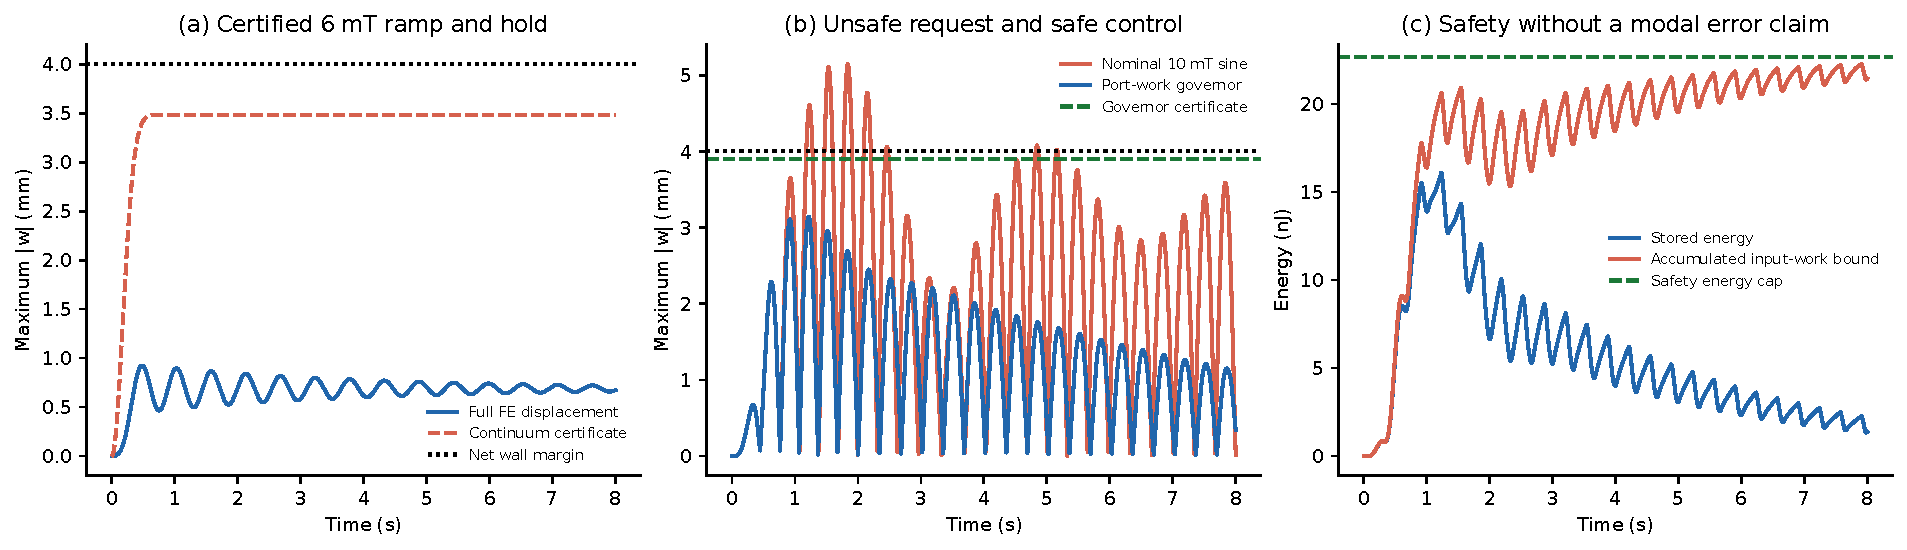
\includegraphics[width=\textwidth]{figures/unified_beam_safety_3panel.pdf}
\caption{Whole-beam safety for the shared full FE plant, with zero initial
energy and default drag.  (a) A $6$ mT monotone ramp and its all-time
continuum energy certificate.  (b) The $10$ mT ramped sinusoidal request
at $9.444949$ rad/s violates the $4$ mm net corridor margin; the actual
port-work governor preserves it with an analytically guaranteed bound.
(c) Stored energy and accumulated input-work bound for the governed case.
The wall half-width is $4.6$ mm and rod radius $0.6$ mm.  These
geometric constraints define the simulated corridor; patient-specific
clearance requires a corresponding geometry and parameter model.}
\label{fig:unifiedsafety}
\end{figure*}

For the $6$ mT sinusoid, the maximum tip discrepancies of the
$2$-, $4$-, and $8$-mode reconstructions against the full $64$-mode FE
trajectory are $22.7168$, $5.9661$, and $1.5156$ $\mu$m, respectively
($0.73510\%$, $0.19306\%$, and $0.04904\%$ of the full-FE peak).
These are measured truncation errors for this input, not rigorous bounds
for all neglected modes or all trajectories.  The full-continuum energy
certificate does not substitute any of them for an unknown error constant.
An independent COMSOL HermitianBeam integration of the same $32$-element
consistent-mass model gives a default-sinusoid peak of $3.09032$ mm;
its largest tip difference from the present integration is $0.11835$
$\mu$m.  Tightening the COMSOL relative tolerance to $10^{-8}$ reduces
the largest tip difference to $0.02160$ $\mu$m.
Independent COMSOL runs also reproduce the $6$ mT monotone-ramp safe case
and $10$ mT sinusoidal violation: their peaks are $0.924046$ and
$5.144787$ mm, with maximum cross-solver tip discrepancies of $0.00663$
and $0.03489$ $\mu$m, respectively.
This cross-check concerns the same mathematical model and does
not calibrate material or actuation parameters against hardware.

The closed-loop governor was also implemented inside COMSOL, coupling a
global ODE for $W/E_{\max}$ to the nonlinear magnetic end moment.
This run used the generalized-$\alpha$ time integrator with
$\rho_\infty=0$, relative tolerance $10^{-5}$, and a maximum internal
step of $0.002$ s; the $2001$ saved outputs are spaced by $0.004$ s.
Its full-FE centerline peak is $3.143643$ mm, leaving a sampled net
clearance of $0.856357$ mm.  The maximum tip discrepancy from the refined
Python trajectory is $0.582073$ $\mu$m, or $0.018516\%$ of its peak.
The applied field remains below $9.816986$ mT.  The COMSOL-integrated
work observer peaks at $22.253032$ nJ, or $0.9818823E_{\max}$;
$E\leq W\leq E_{\max}$ and the magnetic-power projection hold at every
saved time.  Its maximum work-observer discrepancy from Python is
$2.263\times10^{-12}$ J.

For an independent energy ledger, reconstruct $E$ from all displacement
and velocity DOFs and compute
\begin{align*}
 D_h(t)&=\int_0^t\alpha\dot q^{\mathsf T}M\dot q\dd\tau,\\
 R_E(t)&=E(t)-E(0)-[W(t)-W(0)]\\
       &\quad+D_h(t).
\end{align*}
Simpson quadrature on the saved outputs gives
$\max_t|R_E(t)|=5.796\times10^{-12}$ J after rounding up,
or $2.605\times10^{-4}$ of the work scale.
The Simpson--trapezoid difference for that dissipation integral is
$2.424\times10^{-13}$ J.  This COMSOL run uses high-frequency numerical
damping and a looser tolerance than the refined Python integration;
its ledger residual includes time-integration and output-quadrature
errors.  The separately integrated COMSOL work state is used for the
observer comparison, rather than replacing it by a coarse-output input
power integral.  These numerical checks corroborate the implementation;
the continuous-time clearance statement remains the analytic invariant
in Proposition~\ref{prop:unifiedgovernor}.

\begin{figure*}[t]
\centering
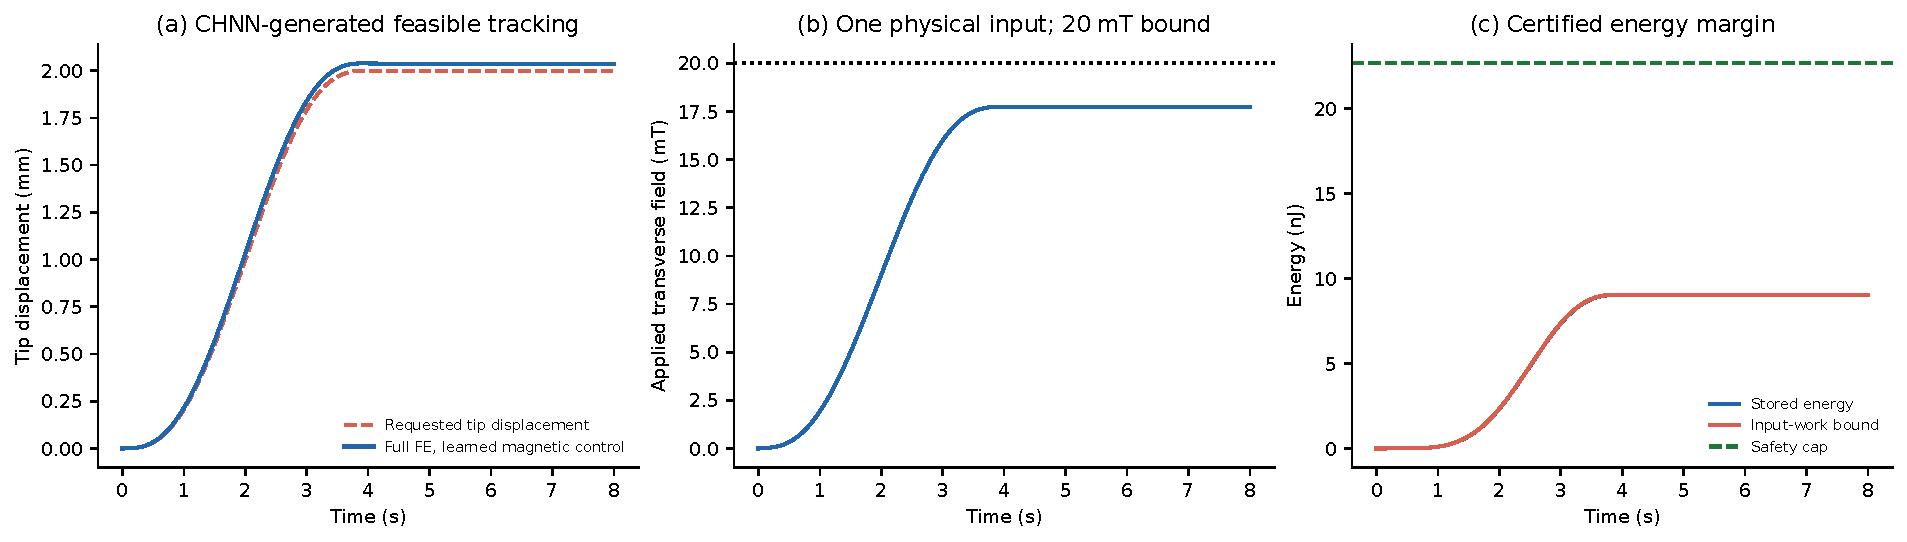
\includegraphics[width=\textwidth]{figures/unified_beam_learned_tracking.pdf}
\caption{The fitted GC17 CHNN and identified drag generate a single
bounded transverse magnetic input for the same full $32$-element FE beam.
(a) A feasible $2$ mm tip request over $4$ s and the actual full-FE tip
motion.  (b) The applied field remains below the declared $20$ mT limit.
(c) Stored energy and the actual-port work observer stay below the safety
cap.  The controller uses the exact first-two-mode projection available in
this simulation; the safety observer uses full-model tip power.
No modal actuation authority or unmeasured-state observer is assumed.
The governor is inactive for this feasible tracking request; its active
effect is tested separately in Figure~\ref{fig:unifiedsafety}.}
\label{fig:unifiedlearnedtracking}
\end{figure*}

\subsection{The learned CHNN generates a feasible magnetic tracking request}
\label{sec:unifiedlearnedcontrol}
To evaluate learned magnetic tracking, the fitted GC model
with seed $17$ and its identified dissipation coefficient generate a nominal
magnetic field for the full FE plant.  Let $z=(X_1,X_2,Y_1,Y_2)$ denote
the observed projection onto the first two static-field modes,
$\ell^{\mathsf T}X$ its reconstructed tip displacement, and
$h_\theta$ the fitted energy, including all learned mixed and
momentum-dependent quartic coefficients.  Define, in the dimensionless
time $\tau=\omega_0t$,
\begin{align}
 y&=\ell^{\mathsf T}X,\qquad
 y'=\ell^{\mathsf T}h_{\theta,Y},\\
 f_0&=\ell^{\mathsf T}h_{\theta,YX}h_{\theta,Y}\notag\\
 &\quad-\ell^{\mathsf T}h_{\theta,YY}
       (h_{\theta,X}+D_\theta h_{\theta,Y}),\\
 g_0&=\ell^{\mathsf T}h_{\theta,YY}d\cos(d^{\mathsf T}X),\\
 D_\theta&=\widehat\gamma\,\diag(\nu)^{-1}.
 \label{eq:unifiedlearnedoutput}
\end{align}
Where $g_0\ne0$, the nominal request is
\begin{align}
 a_r&=r''-k_p(y-r)-k_d(y'-r'),\\
 u_*&=(a_r-f_0)/g_0,\\
 B_{\mathrm{req}}&=B_0\operatorname{clip}_{[-b,b]}(u_*),\\
 b&=B_{\max}/B_0.
 \label{eq:unifiedlearnednominal}
\end{align}
The primes on $r$ denote derivatives in $\tau$.  We use
$k_p=16/\omega_0^2$, $k_d=8/\omega_0$, and
$\widehat\gamma=0.0486617964$.  Both Hessian blocks are evaluated from
the fitted model; they are not replaced by their quadratic-prior values.
The plant receives only the scalar $B_y$ through its actual tip moment,
after the work-governor projection.  It receives no independently
assigned modal forces.

The requested SI tip trajectory is
$y_{\mathrm{ref}}(t)=2\,\mathrm{mm}\,(10s^3-15s^4+6s^5)$ for
$s=t/(4\,\mathrm{s})\in[0,1]$, followed by a hold through $8$ s, and
$r(\tau)=y_{\mathrm{ref}}(\tau/\omega_0)$.
The field limit is $B_{\max}=20$ mT for this separate tracking protocol.
This limit follows from the static input authority: a $2$ mm
equilibrium requires $\vartheta=2y_{\mathrm{tip}}/L=0.05$ and
\begin{equation}
 B_y^{\mathrm{eq}}=
 \frac{EI\vartheta/(\mu L)+B_0\sin\vartheta}{\cos\vartheta}
 \simeq17.43\ \mathrm{mT}.
 \label{eq:unifiedstaticreach}
\end{equation}
The $10$ mT sinusoidal safety tests and the $2$ mm tracking experiment
thus use different input amplitudes, with the tracking limit set by the
required equilibrium field.

On the full $64$-DOF plant, the actual tip has an RMS tracking error of
$33.734$ $\mu$m and a maximum error of $47.069$ $\mu$m.  The final tip
position is $2.03515$ mm and the largest centerline displacement is
$2.03838$ mm.  The applied field peaks at $17.75695$ mT; saturation and
governor intervention occur at $0\%$ of saved times.  Thus the feasible
learned request passes through the filter unchanged, and the separate
unfiltered run is identical.  The input-work bound peaks at $9.05293$ nJ,
below the $22.66365$ nJ cap, and the same continuous-time safety invariant
applies.  The minimum absolute input gain along this run is
$0.0138678$ m, so the division in \eqref{eq:unifiedlearnednominal} does
not approach a singularity.  The physical power-balance residual is
$3.53\times10^{-20}$ J. This tracking result assumes access to the
two-mode projection of the full state. Extending it to incomplete sensing
requires a state observer and a corresponding tracking analysis.



A second run uses the CHNN identified by integral fitting of full-FE
COMSOL displacement and velocity exports, with
cosine multiplier $1.0223248822$. Its complete gradient and Hessian,
including learned momentum quartics, generate the same $2$ mm request
on the same full-FE Python plant. For this conservative fit, a separate
PSD drag identification on the existing Python-generated damped beam
trajectories gives $\widehat\gamma=0.0486617702$; this dissipative
training source is distinct from the COMSOL conservative data.
The tip RMSE is $33.726$ $\mu$m, its maximum error is $47.065$ $\mu$m,
and the largest centerline displacement is $2.038365$ mm.
The applied field peaks at $17.756854$ mT and the work observer at
$9.052842$ nJ. Saturation and governor intervention are again zero at
the saved times, and the physical power-balance residual is
$3.53\times10^{-20}$ J. This COMSOL-trained model and the Python-trained
GC17 model use the same physical plant.
The full-state projection and actual-port measurement assumptions are
unchanged, and the same continuum clearance guarantee applies.

Finally, the single uniform-field dipole supplies one boundary moment.
In static equilibrium with no distributed transverse loading,
$w_{ssss}=0$ and the free-tip shear condition imply
$w(s)=\vartheta s^2/(2L)$.
This one-parameter family cannot realize an arbitrary S-shaped static centerline.
The moving-base endpoint task in Section~\ref{sec:s-path} instead follows an
S-shaped tip history using axial base feed and magnetic bending.
The governor preserves the corridor for feasible magnetic requests.
Prescribing more general static shapes requires additional actuation
authority, such as distributed magnetic moments or independently
controlled loads.
